% !TEX root = thesis.tex
\documentclass[thesis]{subfiles}

\begin{document}
%*******************************************************************************
%*********************************** First Chapter *****************************
%*******************************************************************************

\chapter{Introduction}  %Title of the First Chapter

\begin{chapquote}{Marvin Minsky, \textit{Prologue: A View from 1988, Perceptrons}}
``The marvelous powers of the brain emerge not from any single, uniformly structured connectionist network but from highly evolved arrangements of smaller, specialized networks which are interconnected in very specific ways.''
\end{chapquote}

%********************************** %First Section  **************************************
Deep learning has in recent years come to dominate the previously separate fields of research in machine learning, computer vision, natural language understanding and speech recognition. That these fields would have been considered relatively distinct less than 5 years ago belies the power of the method. Deep learning is only the latest in a long history of connectionist learning research, and while the breakthroughs in training deep networks are real, and the research community has continued to discover increasingly more applications for deep learning, many relatively simple questions of learning in neural networks\index{neural network} remain unanswered.

% Begin research statement stuff
\section{End-to-End Learning}
Classic computer vision approaches depended on hand-designing problem specific \emph{features} --- salient representations of the input --- requiring expert knowledge of the domain, limiting the scalability and effectiveness of this approach. Early computer vision research, for example, depended on finding prominent edges in images. The often cited appeal of deep learning, as compared to classic feature-driven approaches in computer vision (and speech recognition, etc), is that neural networks\index{neural network} are trained `end-to-end', \ie without needing manual design of internal representations. Whereas in classic computer vision, more salient representations of the input must be hand-designed for each problem, deep networks can be trained directly on the original data itself, and have been shown to learn better representations of the data.

\begin{figure}[tbp]
	\centering
	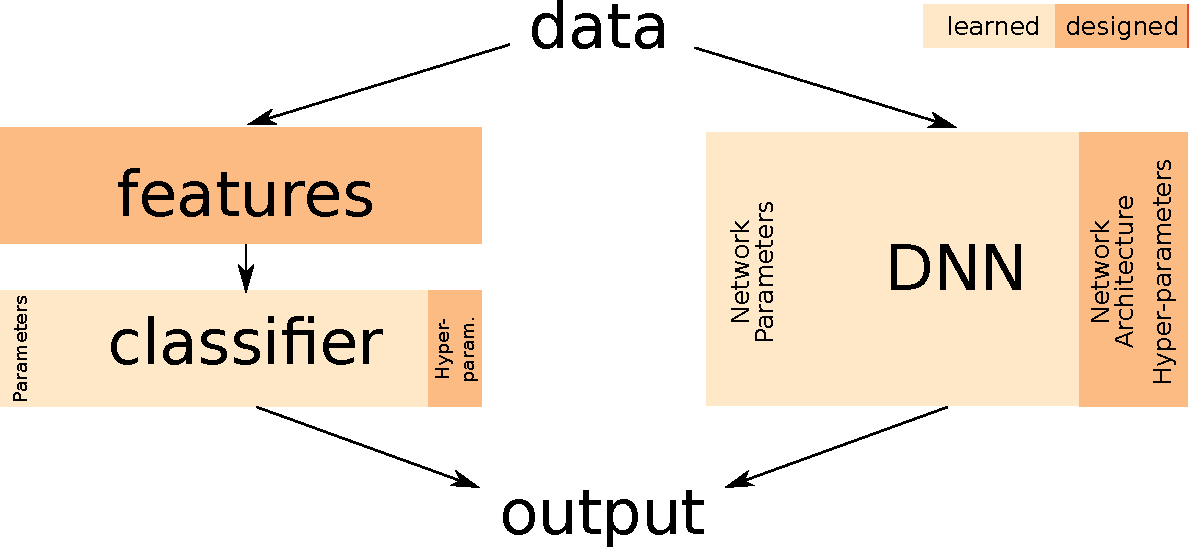
\includegraphics[width=0.9\textwidth]{dnnvsfeatures}
	\caption[Classic feature-based approach \vs{}deep learning.]{\textbf{A comparison of classic feature-based approach to computer vision, and deep learning approaches.} Although both methods require hand-tuned hyper-parameters and design, deep learning methods avoid much of the hand-engineering of classic approaches. Deep networks are far from automatic however, for every application hyper-parameters must be tuned and significant thought has to be put into the design of the structure of the network.}\label{dnnvsfeatures}
\end{figure}
	
Glossed over in this description of deep learning, as it is often in the field itself, is that this learning ability does not come for free, and is far from automatic. It relies on very specific assumptions that are mostly encoded in the design of the neural network\index{neural network} architecture itself --- what, for the sake of brevity, in this thesis we will denote \emph{structural priors}.
%--- perhaps necessitated by the Free Lunch Theorem (see \cref{nofreelunch}).

Structural priors require some knowledge of the domain to design but, unlike hand-designed features, are higher level and have relatively broad applicability. In real-world applications fully-connected neural networks\index{neural network} are seldom used, every practical application of deep learning has relied on some form of structural prior. \Cref{dnnvsfeatures} illustrates, at a high level, the amount of learning \vs{}design in deep learning as compared to traditional feature-based computer vision.

For example, \glspl{cnn} are a broad class of neural network\index{neural network} architectures that encode assumptions based on our prior knowledge about learning with natural image inputs. \Glspl{rnn} are another broad class of architectures that encode our prior knowledge about learning sequence inputs, such as natural language sentences. Neural networks designed with problem-salient structural priors have fewer parameters, are faster, and have better \emph{generalization} --- better accuracy on data outside the training set --- than the fully connected equivalent.
% ------------------------ End research statement stuff

\section{Understanding the Effect of Structure on Learning}
Although it has been proven that a neural network\index{neural network} with an infinitely wide single hidden layer is a universal approximator~\citep{journals/mcss/Cybenko92,hornik89a},  theoretically able to learn any function, in practice the architecture of a neural network\index{neural network} has an unreasonably large affect on the generalization of a trained network. For example, it has been well demonstrated that for image classification, a reasonably designed \gls{cnn} as proposed by \citet{Lecun1998} will always outperform a fully-connected network, no matter the number of hidden units learned. This is despite the fact that, as explained in \cref{background}, any \gls{cnn} can be represented exactly in a (larger) fully connected network where shared parameters are replaced by duplicated weights and filter connectivity is simply represented by zeroed out weights.

Novel work on optimization algorithms used to train neural networks\index{neural network} is considered research progress, while novel structural changes made in deep networks are often dismissed as `engineering', but this is to fundamentally misunderstand the importance of structure. If a structural change results in lower training loss for the same objective and dataset, then it is moving towards understanding the black box internal representation learned in deep networks. %Some of the most consequential recent work in the field, such as residual networks (see \cref{residualnetworks}, fit the description of learning strutural priors. %, sparsifying neural networks\index{neural network} to exploit our prior knowledge of the importance of local correlations in natural images.

This lack of understanding in both the optimization and structure of deep networks has meant that contemporary deep network architectures for image classification have high computational and memory complexity. This is a direct result of the inability to identify the optimal architecture for datasets. The approach advocated by many researchers in the field has been to train monolithic networks with excess complexity, and strong regularization --- an approach that has found success in practice for accuracy, but leaves much to desire in efficiency.

In this thesis we propose that carefully designing networks in consideration of our prior knowledge of the task can improve the memory and compute efficiency of state-of-the art networks, and even increase accuracy through structurally induced regularization. This is not a completely new idea, and received focus in an earlier iteration of connectionist research progress, the late 80's and early 90's --- \gls{cnn} are perhaps the most successful example of this approach --- but it is one that contemporary research in the field often misunderstands the significance of.
\section{Contributions}
While this philosophy defines our approach, deep neural networks\index{neural network} have a large number of degrees of freedom, and there are many facets of deep neural networks\index{neural network} that warrant such analysis. In this thesis, we have looked at several interrelated aspects of deep \gls{cnn}:
\begin{enumerate*}[label=(\textbf{\roman*)}]
\item spatial connectivity (\cref{lowrankfilters}),
\item inter-filter connectivity (\cref{deeproots}),
\item and conditional connectivity (\cref{conditionalnetworks})
\end{enumerate*}.
So as to not conflate the methods and results, we have attempted to present each of these in isolation. 
This thesis is organized as follows:
\begin{description}
	\item[\Cref{background}] gives the necessary background on neural networks\index{neural network}, and contemporary deep learning architectures
	%decision forests and their applications, 
	with particular emphasis on image classification, in order to understand our work and motivation.
	
	\item[\Cref{motivation}] explores the effect of structure on learning in neural networks\index{neural network}, in particular machine learning theory and early practical results towards understanding the effect of the size and structure of neural networks\index{neural network} on their generalization, motivating the focus of this thesis.
	
	\item[\Cref{lowrankfilters}] addresses the spatial extents of convolutional filters, proposing to exploit our knowledge of the low-rank nature of most filters learned for image recognition by structuring a deep network to learn a low-rank basis for filters.
	
	Rather than approximating filters in previously-trained networks with more efficient versions, we learn a set of small basis filters from scratch; during training, the network learns to combine these basis filters into more complex filters that are discriminative for image classification. To train such networks, a novel weight initialization scheme is used. This allows effective initialization of connection weights in convolutional layers composed of groups of differently-shaped filters. 
	
	We validate our approach by applying it to several existing \gls{cnn} architectures and training these networks from scratch using the CIFAR, \gls{ilsvrc} and MIT Places datasets. Our results show similar or higher accuracy than conventional \glspl{cnn} requiring much less compute. %Applying our method to an improved version of VGG-11 network using global max-pooling, we achieve comparable validation accuracy using 41\% less compute and only 24\% of the original VGG-11 model parameters; another variant of our method gives a 1 percentage point {\em increase} in accuracy over our improved VGG-11 model, giving a top-5 \emph{center-crop} validation accuracy of 89.7\% while reducing computation by 16\% relative to the original VGG-11 model. Applying our method to the GoogLeNet architecture for \gls{ilsvrc}, we achieved comparable accuracy with 26\% less compute and 41\% fewer model parameters. Applying our method to a near state-of-the-art network for CIFAR, we achieved comparable accuracy with 46\% less compute and 55\% fewer parameters. 
	
	\item[\Cref{deeproots}] addresses the filter/channel extents of convolutional filters, by learning filters with limited channel extents. A new method for creating computationally efficient and compact \glspl{cnn} using a novel sparse connection structure that resembles a tree root. This allows a significant reduction in computational cost and number of parameters of state-of-the-art deep \glspl{cnn} without compromising accuracy. 
	
	We validate our approach by using it to train more efficient variants of state-of-the-art \gls{cnn} architectures, evaluated on the \gls{cifar10} and \gls{ilsvrc} datasets. Our results show similar or higher accuracy than the baseline architectures with much less compute. %, as measured by \gls{cpu} and \gls{gpu} timings. For example, for ResNet 50, our model has 40\% fewer parameters, 45\% fewer floating point operations, and is 31\% (12\%) faster on a \gls{cpu} (\gls{gpu}). For the deeper ResNet 200 our model has 25\% fewer floating point operations and 44\% fewer parameters, while maintaining state-of-the-art accuracy. For GoogLeNet, our model has 7\% fewer parameters and is 21\% (16\%) faster on a \gls{cpu} (\gls{gpu}).
	
	\item[\Cref{conditionalnetworks}] presents work towards conditional computation in deep neural networks\index{neural network}, conditional networks, allowing for faster inference, by understanding the connections between two state of the art classifiers: \glspl{dnn} and randomized decision forests.
	
	We propose a new discriminative learning model, \emph{conditional networks}, 
	that jointly exploits the accurate \emph{representation learning} capabilities of deep neural networks\index{neural network} with the efficient \emph{conditional computation} of decision trees and directed acyclic graphs (DAGs).
	Conditional networks can be thought of as a way to learn an optimal block-diagonal sparsification of a \gls{dnn}, and we show how they can be trained to cover the continuous spectrum between deep networks and decision forests/jungles. 
	
	In addition to improving test and training efficiency, conditional networks yield smaller models, are highly interpretable, and offer test-time flexibility. Validation is performed on standard image classification tasks. Compared to the state of the art, our results demonstrate superior efficiency for at-par accuracy both on the ImageNet and CIFAR datasets.
	
	\item[\Cref{conclusion}] summarizes the contributions made in this thesis, and reviews the results.
	
	\item[\Cref{futurework}] looks at the research questions that arise from the work presented in this thesis, in particular the importance of the significant hand-design still present in ``end-to-end'' learning, the effectiveness of structural priors, the and ineffectiveness of current optimization methods. Proposals are made for future research directions which seem pertinent given our results.
	
\end{description}

\end{document}
